
%% This is file `sample-acmsmall.tex',
%% generated with the docstrip utility.
%%
%% The original source files were:
%%
%% samples.dtx  (with options: `acmsmall')
%% 
%% IMPORTANT NOTICE:
%% 
%% For the copyright see the source file.
%% 
%% Any modified versions of this file must be renamed
%% with new filenames distinct from sample-acmsmall.tex.
%% 
%% For distribution of the original source see the terms
%% for copying and modification in the file samples.dtx.
%% 
%% This generated file may be distributed as long as the
%% original source files, as listed above, are part of the
%% same distribution. (The sources need not necessarily be
%% in the same archive or directory.)
%%
%% The first command in your LaTeX source must be the \documentclass command.
\documentclass[sigplan,screen]{acmart}
\usepackage{booktabs}
\usepackage{listings}
\usepackage{tcolorbox}
\usepackage{tikz}
\usepackage{tkz-graph}
\usepackage{stmaryrd}
\usepackage{amsmath}

% \lstset{basicstyle=\ttfamily}
\usetikzlibrary{shapes.geometric, arrows}

\tikzstyle{startstop} = [rectangle, rounded corners, minimum width=3cm, minimum height=1cm,text centered, draw=black, fill=red!30]
\tikzstyle{process} = [rectangle, minimum width=3cm, text width=0.3*\columnwidth, minimum height=1cm, text centered, draw=black, fill=orange!30]
\tikzstyle{decision} = [diamond, minimum width=3cm, minimum height=1cm, text centered, draw=black, fill=green!30]
\tikzstyle{arrow} = [thick,->,>=stealth]

\lstset{language=haskell, deletekeywords={abs},basicstyle=\ttfamily}

\newcommand{\expr}[1]{(#1)} % Expression quasiquote
\newcommand{\rarr}{\rightarrow}
\newcommand{\Rarr}{\Rightarrow}
\newcommand{\rewrites}{\Longrightarrow}

\newcommand{\typeeq}{\raise.17ex\hbox{$\scriptstyle\mathtt{\sim}$}\,\;}

\newcommand{\ttt}{\texttt}

\newenvironment{todo}
  {\begin{tcolorbox}
   \textbf{TODO}:
  }
  {\end{tcolorbox}
  }

% \newenvironment<>{todo}[1][]{
%     \setbeamercolor{block body example}{fg=black,bg=blue}
%     \setbeamercolor{block title example}{fg=white,bg=red!75!black}
%     \setbeamertemplate{blocks}[rounded][shadow=false]
%   \begin{todo}[]}{\end{todo}
% }

%%
%% \BibTeX command to typeset BibTeX logo in the docs
\AtBeginDocument{%
  \providecommand\BibTeX{{%
    \normalfont B\kern-0.5em{\scshape i\kern-0.25em b}\kern-0.8em\TeX}}}

%% Rights management information.  This information is sent to you
%% when you complete the rights form.  These commands have SAMPLE
%% values in them; it is your responsibility as an author to replace
%% the commands and values with those provided to you when you
%% complete the rights form.
\setcopyright{acmcopyright}
\copyrightyear{2020}
\acmYear{2020}
\acmDOI{1}


%% These commands are for a PROCEEDINGS abstract or paper.
\acmConference[Haskell '20]{Haskell '20: Proceedings of the 13th
  ACM SIGPLAN International Symposium on Haskell}{August 27 -- 28, 2020}{New Jersey, United States,}
\acmBooktitle{Haskell '20: ACM SIGPLAN International Symposium on Haskell,
  August 27 -- 28, 2020, New Jersey, United States}
\acmPrice{15.00}
\acmISBN{978-1-4503-XXXX-X/18/06}


%%
%% Submission ID.
%% Use this when submitting an article to a sponsored event. You'll
%% receive a unique submission ID from the organizers
%% of the event, and this ID should be used as the parameter to this command.
%%\acmSubmissionID{123-A56-BU3}

%%
%% The majority of ACM publications use numbered citations and
%% references.  The command \citestyle{authoryear} switches to the
%% "author year" style.
%%
%% If you are preparing content for an event
%% sponsored by ACM SIGGRAPH, you must use the "author year" style of
%% citations and references.
%% Uncommenting
%% the next command will enable that style.
%%\citestyle{acmauthoryear}

%%
%% end of the preamble, start of the body of the document source.
\begin{document}

%%
%% The "title" command has an optional parameter,
%% allowing the author to define a "short title" to be used in page headers.
\title{Title Goes Here}

%%
%% The "author" command and its associated commands are used to define
%% the authors and their affiliations.
%% Of note is the shared affiliation of the first two authors, and the
%% "authornote" and "authornotemark" commands
%% used to denote shared contribution to the research.
\author{David Young}
\email{d063y800@ku.edu}

% \authornote{Both authors contributed equally to this research.}
% \email{trovato@corporation.com}
% \orcid{1234-5678-9012}

\author{Andrew Gill}
\email{andygill@ku.edu}

%%
%% By default, the full list of authors will be used in the page
%% headers. Often, this list is too long, and will overlap
%% other information printed in the page headers. This command allows
%% the author to define a more concise list
%% of authors' names for this purpose.
% \renewcommand{\shortauthors}{Trovato and Tobin, et al.}
\renewcommand{\shortauthors}{Young and Gill}

%%
%% The abstract is a short summary of the work to be presented in the
%% article.
\begin{abstract}
  Domain specific languages (DSLs) provide a powerful tool for to abstract over
  a class of problems. In this paper, we introduce a technique for representing
  algebraic data types and pattern matching in a DSL embedded in Haskell. This
  representation is mechanized through the use of GHC Generics and and GHC Core plugin.
\end{abstract}

\begin{CCSXML}
<ccs2012>
   <concept>
       <concept_id>10011007.10011006.10011050.10011017</concept_id>
       <concept_desc>Software and its engineering~Domain specific languages</concept_desc>
       <concept_significance>500</concept_significance>
       </concept>
 </ccs2012>
\end{CCSXML}

\ccsdesc[500]{Software and its engineering~Domain specific languages}

% \keywords{domain specific languages}

%%
%% The code below is generated by the tool at http://dl.acm.org/ccs.cfm.
%% Please copy and paste the code instead of the example below.
%%
% \begin{CCSXML}
% <ccs2012>
%  <concept>
%   <concept_id>10010520.10010553.10010562</concept_id>
%   <concept_desc>Computer systems organization~Embedded systems</concept_desc>
%   <concept_significance>500</concept_significance>
%  </concept>
%  <concept>
%   <concept_id>10010520.10010575.10010755</concept_id>
%   <concept_desc>Computer systems organization~Redundancy</concept_desc>
%   <concept_significance>300</concept_significance>
%  </concept>
%  <concept>
%   <concept_id>10010520.10010553.10010554</concept_id>
%   <concept_desc>Computer systems organization~Robotics</concept_desc>
%   <concept_significance>100</concept_significance>
%  </concept>
%  <concept>
%   <concept_id>10003033.10003083.10003095</concept_id>
%   <concept_desc>Networks~Network reliability</concept_desc>
%   <concept_significance>100</concept_significance>
%  </concept>
% </ccs2012>
% \end{CCSXML}

% \ccsdesc[500]{Computer systems organization~Embedded systems}
% \ccsdesc[300]{Computer systems organization~Redundancy}
% \ccsdesc{Computer systems organization~Robotics}
% \ccsdesc[100]{Networks~Network reliability}

%%
%% Keywords. The author(s) should pick words that accurately describe
%% the work being presented. Separate the keywords with commas.
% \keywords{datasets, neural networks, gaze detection, text tagging}


%%
%% This command processes the author and affiliation and title
%% information and builds the first part of the formatted document.
\maketitle

\section{Introduction}

Embedded domain specific languages (EDSLs) have long been an effective
technique for constructing reusable tools for working in a variety of
different problem domains. Haskell is a language which is particularly
well-suited to EDSLs due to its lazy evaluation, first-class functions and
lexical closures.

Despite these advantages Haskell provides for creating EDSLs, there are a few
constructs for which representations have proven illusive. One prominent example
is that of a \ttt{case} expression. Pattern matching is a convenient way to
implement control flow structures and to view components of data structures, so
it is frequently a desirable feature for many EDSLs.

Additionally, lambdas can also be difficult to implement in EDSLs. A major reason
for this is that control flow constructs which are typically \textit{outside} the EDSL,
such as pattern matching and tail recursion, can make it challenging to "look inside"
the lambda.

The following contributions are made by this paper:

\begin{itemize}
\item A representation of pattern matching in a Haskell EDSL (Section 3)
\item Representations of tail recursion (Section 4) and lambdas (Section 5) in
  the EDSL. We will see that lambdas become easier to implement once pattern
  matching and tail recursion already have EDSL representations.
\item A GHC Core plugin which transforms a subset of standard Haskell code
  into this EDSL for pattern matching, extended with tail recursion,
  lambdas and primitive operations (Section 7)
\item An implementation of a interpreter for the "standard" semantics of the EDSL (Section 6).
\end{itemize}

\subsection{Overview}

In this EDSL, the type representing values in the expression language is \ttt{E t}
and there are two basic functions which translate values to and from this
expression language with the following type signatures:

\begin{lstlisting}
rep :: a -> E a
abs :: E a -> a
\end{lstlisting}

In this paper, the data constructors of the \ttt{E} type will be described
incrementally as they are needed.

\subsection{Translation Example}
\begin{todo}
  Does it make sense for this to be a subsection of the intro?
\end{todo}

In the example below, the Core plugin transforms \ttt{example} into \ttt{example'}:
\begin{lstlisting}[deletekeywords={Ord}]
import Data.Char (ord)

x :: Either Char Int
x = Left 'a'

example :: Int
example =
  internalize (externalize
    (case x of
      Left  c -> ord c
      Right i -> i))

example' :: Int
example' =
  abs (CaseExp
        (rep x)
        (SumMatchExp (OneProdMatch
                       (Lam 1
                         (Ord (Var 1))))
                     (OneSumMatch
                       (OneProdMatch
                         (Lam 2
                           (Var 2)))))
\end{lstlisting}

[\ldots]

\section{Representing Algebraic Datatypes}

Briefly, a algebraic type \ttt{T} with an automatically generated \ttt{ERep}
instance is given a representation in terms of \ttt{Either}, \ttt{(,)}, \ttt{()}
and \ttt{Void}.  This "standardized" type representation is given by \ttt{ERepTy
T}. \ttt{ERepTy} is an type family associated to the type class \ttt{ERep}. This
type will be called the \textit{canonical type} of \ttt{T}.

Only the "outermost" type will be deconstructed into these fundamental building
blocks, and further deconstruction can take place on these pieces later on. For
example, consider this type:

\begin{lstlisting}
data ComplexPair where
  ComplexPair :: Complex Double
                 -> Complex Double
                 -> ComplexPair
  deriving (Generic, Eq, Show)

instance ERep ComplexPair
\end{lstlisting}

Note that the instance definition is automatically generated from the
\ttt{Generic} instance.

Given this code, \ttt{ERep ComplexPair \typeeq (Complex Double, Complex Double)}. Here
is an example that demonstrates why this is more useful than if it \textit{fully} deconstructed
each type into \ttt{Either}, \ttt{(,)} and \ttt{()}:

\begin{lstlisting}
sumComplexPair ::
  ComplexPair -> Complex Double
sumComplexPair p =
  internalize (externalize
    (case p of
      ComplexPair a b -> a + b))
\end{lstlisting}

If \ttt{ERep ComplexPair} were fully deconstructed into \ttt{((Double, Double),
(Double, Double))}, we would need a \ttt{Num} instance for \ttt{(Double,
Double)}.  What we really want is to use the fact that a \ttt{Num} instance
already exists for \ttt{Complex Double}. This is exactly what preserving this
type information allows us to do.

It is important to note that we are still able to further deconstruct this type
with further pattern matches, since \ttt{ERep (Complex Double) \typeeq (Double, Double)}:

\begin{lstlisting}
realSum :: ComplexPair -> Double
realSum p =
  internalize (externalize
    (case p of
      ComplexPair a b ->
        case a of
          a_real :+ _ ->
            case b of
              b_real :+ _ ->
                a_real + b_real))
\end{lstlisting}

\begin{todo}
  Should we use a single nested pattern match in the above block? Both
  are functional (and equivalent) from a technical perspective.
\end{todo}

An additional benefit of this is that recursive types require no special handling. For
example, consider:

\begin{lstlisting}
data IntList = Nil | Cons Int IntList
  deriving (Generic, Show)

instance ERep IntList
\end{lstlisting}

Note that \ttt{ERepTy IntList \typeeq Either () (Int, IntList)}. If \ttt{ERepTy}
attempted to "fully deconstruct" \ttt{IntList}, it would send the compiler
into an infinite loop.

This allows us to implement functions on such recursive types:

\begin{lstlisting}
isEmpty :: IntList -> Bool
isEmpty t =
  internalize (externalize
    (case t of
      Nil -> True
      Cons x xs -> False))

intListSum_helper :: (Int, IntList) -> Int
intListSum_helper p =
  internalize (externalize
    (case p of
       (acc, t) ->
         case t of
           Nil -> acc
           Cons x xs ->
             intListSum_helper (x+acc, xs)))

intListSum :: IntList -> Int
intListSum t =
  internalize (externalize
    (intListSum_helper (0, t)))
\end{lstlisting}


\subsection{GHC Generics \ttt{Rep}}

[Remove metadata from Generic representation and turn tree-like structure into a (nested) list-like structure]

\subsection{\ttt{E}, \ttt{ERep}, \ttt{ERepTy}}

There are three interconnected foundational parts: \ttt{E}, \ttt{ERep} and
\ttt{ERepTy}. \ttt{E} is the deep embedding of the EDSL (a GADT that encodes
expressions in the DSL language). \ttt{ERep} is a type class which represents
all Haskell types which can be represented in the DSL. \ttt{ERepTy} is a type
family associated to the \ttt{ERep} type class, which represents a "canonical form"
of the given type. This canonical form can be immediately constructed in the EDSL.
Canonical form types crucially include \ttt{Either} and \ttt{(,)}, which
allow all combinations of basic sum types and product types to be encoded. More
information on this encoding is given in [a different section].

This information is brought into the \ttt{E} type via the constructor
\ttt{Repped}. The \ttt{E} also contains constructors representing \ttt{Either}
and \ttt{(,)} values:

\begin{lstlisting}
data E t where
  ...
  Repped :: ERep t => ERepTy t -> E t

  LeftExp :: E a -> E (Either a b)
  RightExp :: E b -> E (Either a b)

  PairExp :: E a -> E b -> E (a, b)
  ...
\end{lstlisting}

\ttt{ERep} and \ttt{ERepTy} provide an interface for transferring values between the EDSL
expression language and the source Haskell language:

\begin{lstlisting}
class ERep t where
  type ERepTy t

  rep :: t -> E t
  rep = Repped . rep'

  unrep :: ERepTy t -> t

  rep' :: t -> ERepTy t
\end{lstlisting}

The key algebraic instances mentioned before are as follows:

\begin{lstlisting}
instance (ERep a, ERep b)
  => ERep (Either a b) where

  type ERepTy (Either a b) = Either a b

  rep (Left x)  = LeftExp (rep x)
  rep (Right y) = RightExp (rep y)

  unrep = id
  rep'  = id

instance (ERep a, ERep b)
  => ERep (a, b) where

  type ERepTy (a, b) = (a, b)

  rep (x, y) = PairExp (rep x) (rep y)
  unrep = id
  rep'  = id
\end{lstlisting}


\section{Representing pattern matches}

Within the \ttt{E} expression language, a pattern match is represented by the
\ttt{CaseExp} constructor:

\begin{lstlisting}
data E t where
  ...
  CaseExp ::
    (ERep t, ERepTy (ERepTy t) ~ ERepTy t)
      => ERep t
         -> E (SumMatch (ERepTy t) r)
         -> E r
  ...
\end{lstlisting}

The equality constraint ensures that a canonical type is its own canonical type.

\begin{todo}
  Should we make a synonym for this constraint since it is used in
multiple places? Like this:
\begin{lstlisting}
type CanonicalIsIdem t =
  ERepTy (ERepTy t) ~ ERepTy t
\end{lstlisting}
\end{todo}

(The above code block is a slight simplification of the actual implementation,
which has an additional type variable which is used at an "intermediate" point.
The expanded form is in place to simplify the Core transformation.)

The type \ttt{SumMatch} is defined as

\begin{lstlisting}
newtype SumMatch a b =
  MkSumMatch { runSumMatch :: a -> b }
\end{lstlisting}

For the moment, we will primarily use this type as a type tag and ignore
the values it can take on.

A value of type \ttt{E (SumMatch a b)} represents a computation within the EDSL
which destructures a value of type \ttt{E a} and produces a value of type \ttt{E b}.
Therefore, \ttt{E (SumMatch (ERepTy t) r)} represents a computation which destructures
a value of type \ttt{E (ERepTy t)} and produces a value of type \ttt{E b}.



\subsection{\ttt{E (SumMatch a b)}}

The overall structure of a \ttt{E (SumMatch a b)} value is a (heterogeneous)
list of \ttt{E (ProdMatch x y)} values.  Each item of this list corresponds
exactly to one branch in the original \ttt{case} match.

The following constructors generate \ttt{SumMatch}-tagged values in the
expression language:

\begin{lstlisting}
data E t where
  ...
  SumMatchExp ::
    (ERep a, ERep b, ERepTy b ~ b)
      => E (ProdMatch a r)
         -> E (SumMatch b r)
         -> E (SumMatch (Either a b) r)

  OneSumMatch ::
    (ERep a, ERep b, ERepTy a ~ a)
      => E (ProdMatch a b)
         -> E (SumMatch a b)


  EmptyMatch ::
    (ERep b) => E (SumMatch Void b)
  ...
\end{lstlisting}

Note the \ttt{ERepTy a \typeeq a} constraints. This constraint ensures that the type
\ttt{a} is already in canonical form (that is, consists entirely of
\ttt{Either}, \ttt{(,)} and base types).

\subsection{\ttt{E (ProdMatch s t)}}

\ttt{E (ProdMatch x y)} is equivalent to a curried function from \ttt{x} to
\ttt{y} in the expression language .  Note that \ttt{s} is a (potentially
nested) pair type. For example, \ttt{E (ProdMatch (a, (b, c)) r)} is
equivalent to \ttt{E (a -> b -> c -> r)}.

\begin{lstlisting}
data E t where
  ...
  ProdMatchExp ::
    (ERep a, ERep b)
      => E (a -> ProdMatch b r)
         -> E (ProdMatch (a, b) r)

  NullaryMatch ::
    (ERep a)
      => E r -> E (ProdMatch a r)


  OneProdMatch ::
    (ERep a)
      => E (a -> b) -> E (ProdMatch a b)
  ...
\end{lstlisting}

The \ttt{ProdMatch} type is defined similarly to the \ttt{SumMatch} type and is
similiarly used primarily as a type tag:

\begin{lstlisting}
newtype ProdMatch a b =
  MkProdMatch { runProdMatch :: a -> b }
\end{lstlisting}

\subsection{Connection to Church encodings}
\begin{todo}
  Write this subsection
\end{todo}

\subsection{An aside on \ttt{ProdMatch} and \ttt{SumMatch} values}

Though \ttt{ProdMatch} and \ttt{SumMatch} are used throughout this EDSL as type
tags, they do have values and they are not trivial values. The reason for this
is that it connects the encoded pattern matches (values from the \ttt{E}) type
to their semantics. A value of type \ttt{E (SumMatch a b)} is an expression
which takes in a value of type \ttt{a} (embedded within the expression
language), internally performs some pattern matching, and produces a value of
type \ttt{b} (again, embedded within the expression language). This is exactly
the semantics of a function from \ttt{a} to \ttt{b}. Likewise for \ttt{ProdMatch a b}.

Recall the previously mentioned function

\begin{lstlisting}
abs :: E a -> a
\end{lstlisting}

Now consider at the type of \ttt{abs} when it is specialized to take
\ttt{E (SumMatch a b)} values:

\begin{lstlisting}
abs :: E (SumMatch a b) -> SumMatch a b
\end{lstlisting}

If we postcompose with \ttt{runSumMatch}, we get:

\begin{lstlisting}
runSumMatch . abs :: E (SumMatch a b) -> (a -> b)
\end{lstlisting}

The \ttt{SumMatch a b} value which \ttt{abs} returns is exactly the function
which pattern matches according to its input value.

Likewise for \ttt{ProdMatch a b} values.

\section{Representing tail recursion}
\begin{todo}
  Expand the explanation in this section
\end{todo}

\begin{lstlisting}
data Iter a b = Step b | Done a
  deriving (Functor, Generic)

runIter :: (ERep a, ERep b)
  => (a -> Iter b a)
     -> (a -> b)
runIter f = go
  where
    go x =
      case f x of
        Done r  -> r
        Step x' -> go x'
\end{lstlisting}

In the \ttt{E} type, this is used to represent tail recursion by
the following constructors:

\begin{lstlisting}
data E t where
  ...
  StepExp :: E b -> E (Iter a b)
  DoneExp :: E a -> E (Iter a b)

  TailRec :: (ERep a, ERep b)
               => E (b -> Iter a b)
                  -> E (b -> a)
  ...
\end{lstlisting}

\section{Representing lambdas}
This representation of pattern matching depends on the ability to bring
function values into the expression language. This is accomplished
with the following constructors:

\begin{lstlisting}
data E t where
  ...
  Lam ::
    (ERep a, Typeable a)
      => Name a -> E b -> E (a -> b)

  Var :: (Typeable a) => Name a -> E a
\end{lstlisting}

The \ttt{Typeable} constraints are necessary to lookup correctly typed
values in the variable binding environment later on.

The \ttt{Name t} type represents a lambda variable identifier together with its
type \ttt{t} (Note that the \ttt{ScopedTypeVariables} extension is enabled.):

\begin{lstlisting}
newtype Name a = Name Int
  deriving (Eq, Show)

namesEq :: forall a b.
  (Typeable a, Typeable b)
    => Name a -> Name b -> Maybe (a :~: b)
namesEq (Name n) (Name n') =
  case eqT :: Maybe (a :~: b) of
    Just Refl
      | n == n' -> Just Refl
      | otherwise -> Nothing
    Nothing   -> Nothing
\end{lstlisting}

In the Core transformation, each lambda is given a \ttt{Name} with a globally
unique \ttt{Int}, sidestepping any name capture issues.

The following datatypes are used to represent a variable binding environment
of typed names to expression language values:

\begin{lstlisting}
data EnvMapping where
  (:=>) :: forall a.
    Typeable a
    => Name a -> E a -> EnvMapping
\end{lstlisting}

This type encodes a single variable binding, with values of the form
\ttt{n :=> v}, where \ttt{n} is a typed name and \ttt{v} is the value it is bound to.

These bindings are grouped together in the \ttt{Env} type:

\begin{lstlisting}
newtype Env = Env [EnvMapping]

emptyEnv :: Env
emptyEnv = Env []

extendEnv :: Env -> EnvMapping -> Env
extendEnv (Env maps) m = Env (m:maps)

envLookup :: Typeable a
  => Env -> Name a -> Maybe (E a)
envLookup (Env maps) = go maps
  where
    go []                = Nothing

    go ((n' :=> e):rest) =
      case namesEq n n' of
        Just Refl -> Just e
        Nothing   -> go rest
\end{lstlisting}


\section{Recovering standard semantics for pattern matches}

\begin{lstlisting}
abs :: forall t. E t -> t
abs = absEnv emptyEnv

sumMatchAbs ::
  (ERepTy (ERepTy s) ~ ERepTy s, ERep s)
  => Env
    -> E (SumMatch (ERepTy s) t)
    -> s
    -> t
...

prodMatchAbs :: (ERep s)
  => Env
     -> E (ProdMatch s t)
     -> s
     -> t
...

absEnv :: forall t. Env -> E t -> t
absEnv env (CaseExp x f) =
  sumMatchAbs f (absEnv env x)

absEnv env (TailRec f) = \ x ->
  case absEnv env f x of
    Step x' -> absEnv env (TailRec f) x'
    Done r  -> r

absEnv env (Var v) =
  case envLookup env v of
    Just x -> absEnv env
    Nothing ->
      error
        ("No binding for name "
          ++ show v)

absEnv env (Lam (name :: Name a)
                (body :: E b)) =
  \ (arg :: a) ->
    let go :: forall x. E x -> E x
        go expr@(Var name2 :: E a') =
          case namesEq name name2 of
            Just Refl -> rep arg
            _ ->
              case envLookup env name2 of
                Just v  -> v
                Nothing -> expr

        -- [... traverse rest of expression
        --      in go ...]
    in
    absEnv (extendEnv env
                      (name :=> rep arg))
           (go body)

absEnv env (LeftExp x) =
  Left (absEnv env x)

absEnv env (RightExp y) =
  Right (absEnv env y)

absEnv env (PairExp x y) =
  (absEnv env x, absEnv env y)

absEnv env (Repped x) = unrep x

...
\end{lstlisting}


\section{Core Plugin}

The Core plugin translates marked expressions. Expressions are marked by
the \ttt{externalize} function:

\begin{lstlisting}
externalize :: a -> E a
\end{lstlisting}

So, \ttt{externalize x} marks the expression \ttt{x}.

If an expression already has an EDSL type (a type of the form \ttt{E a} for some
\ttt{a}), then the marking procedure ignores it and does not wrap it with
\ttt{externalize} (see $M$ in Section 7.2).

\clearpage
\subsection{Overall Control Flow of the Core Plugin}

In the following flowchart, the names in parentheses in a node refers to the names of transformations from the following section (Section 7.2).

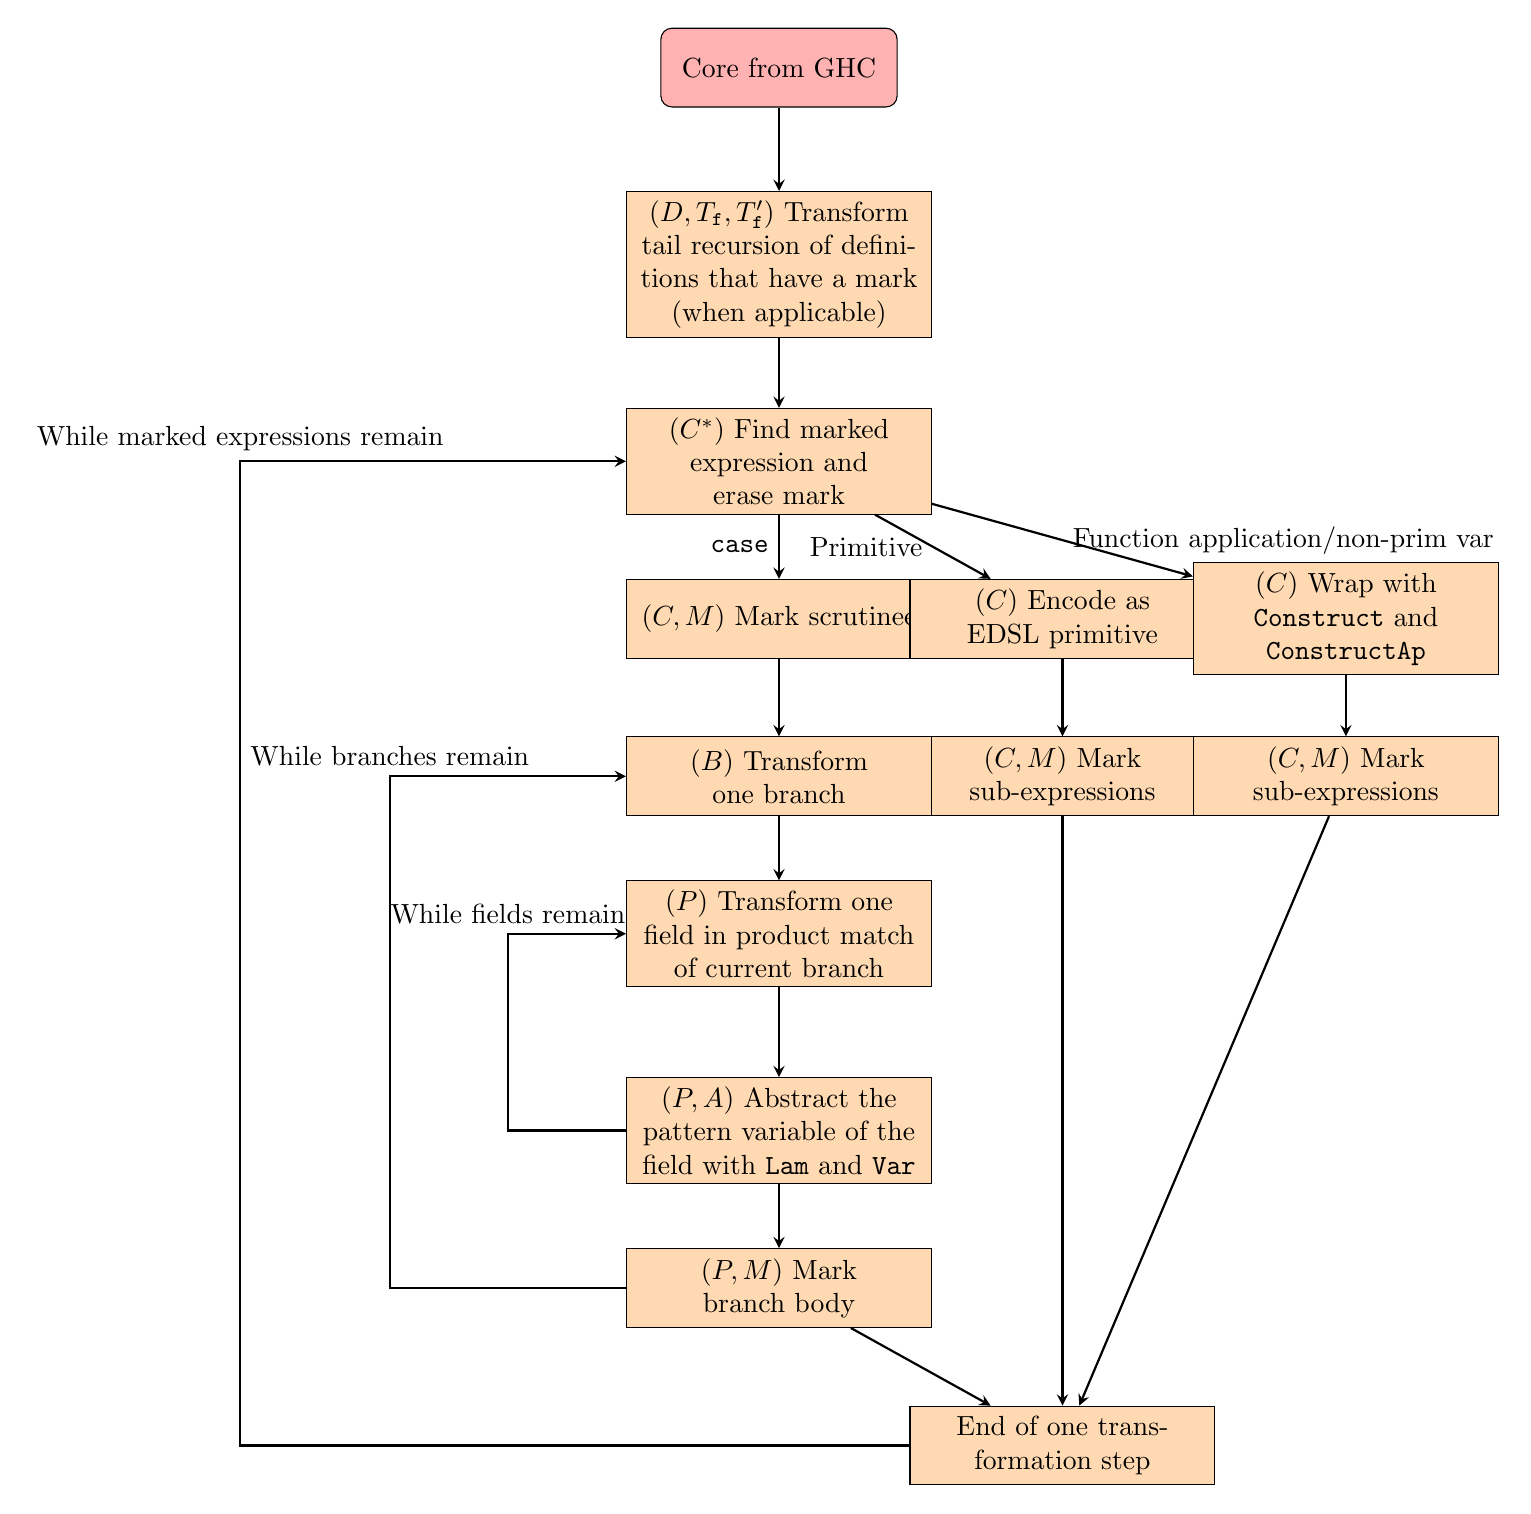
\begin{tikzpicture}[node distance=2cm]
\node (start) [startstop] {Core from GHC};
  \node (tailrec) [process, below of=start, yshift=-0.5cm]{($D, T_{\ttt{f}}, T'_{\ttt{f}}$) Transform tail recursion of definitions that have a mark (when applicable)};
  \node (findmark) [process, below of=tailrec, yshift=-0.5cm]{($C^*$) Find marked expression and erase mark};
    \node (handlecase) [process, below of=findmark]{($C, M$) Mark scrutinee};
    \node (handleprim) [process, right of=handlecase, xshift=1.6cm]{($C$) Encode as EDSL primitive};
    \node (handleapp) [process, right of=handleprim, xshift=1.6cm]{($C$) Wrap with \ttt{Construct} and \ttt{ConstructAp}};

    \node (marksubs1) [process, below of=handleprim]{($C, M$) Mark sub-expressions};
    \node (marksubs2) [process, below of=handleapp]{($C, M$) Mark sub-expressions};

    \node (onebranch) [process, below of=handlecase]{($B$) Transform one branch};
    \node (prodmatch) [process, below of=onebranch]{($P$) Transform one field in product match of current branch};
    \node (abstractvar) [process, below of=prodmatch, yshift=-0.5cm]{($P, A$) Abstract the pattern variable of the field with \ttt{Lam} and \ttt{Var}};
    \node (markbody) [process, below of=abstractvar]{($P, M$) Mark branch body};
    \node (endstep) [process, below of=markbody, right of=markbody, xshift=1.6cm]{End of one transformation step};

  \draw [arrow] (start) -- (tailrec);
  \draw [arrow] (tailrec) -- (findmark);
  \draw [arrow] (findmark) -- node[anchor=east] {Primitive} (handleprim);
  \draw [arrow] (findmark) -- node[anchor=west] {Function application/non-prim var} (handleapp);
  \draw [arrow] (findmark) -- node[anchor=east] {\ttt{case}} (handlecase);

  \draw [arrow] (handleprim) -- (marksubs1);

  \draw [arrow] (handleapp) -- (marksubs2);

  \draw [arrow] (handlecase) -- (onebranch);
  \draw [arrow] (onebranch) -- (prodmatch);
  \draw [arrow] (prodmatch) -- (abstractvar);
  \draw [arrow] (abstractvar) -- (markbody);

  \draw [arrow] (marksubs1) -- (endstep);
  \draw [arrow] (marksubs2) -- (endstep);
  \draw [arrow] (markbody) -- (endstep);


  % \draw (prodmatch) edge[bend right, left] node {While fields remain} (abstractvar);
  % \draw [arrow] (abstractvar.east) to ++(0.5,0) |- node[anchor=west] {While fields remain} (prodmatch.east);
  \draw [arrow] (abstractvar.west) -| ++(-1.5,0) |- node[anchor=south] {While fields remain} (prodmatch.west);

  \draw [arrow] (markbody.west) -| ++(-3,0) |- node[anchor=east, anchor=south] {While branches remain} (onebranch.west);

  \draw [arrow] (endstep.west) -| ++(-8.5,0) |- node[anchor=west, anchor=south] {While marked expressions remain} (findmark.west);

  % \draw (findmark)  edge[loop left] node {While marked expressions remain} (findmark);

  % \draw (findmark)  edge[loop left] node {While marked expressions remain} (findmark);
  % \draw (onebranch) edge[loop left] node {While branches remain} (onebranch);
  % \Loop[label=\(While\, fields\, remain\), labelstyle={left=5pt}](prodmatch);
  % \path (bodylam) edge [left] (onebranch);
  % \path (bodylam) edge [loop above] node {test} (onebranch);
  % \Loop[label=\(While\, remaining\, branches\, exist\), labelstyle={left=5pt}](onebranch)
  % \draw [arrow] (bodylam) -- (onebranch);
  % \draw [arrow] (bodylam.east) to  ++ (1.5,0) |- node[anchor=south] {While branches remain} (onebranch);
  % \draw [arrow] (bodylam.east) to  ++ (1.5,0) |- node[anchor=south] {While branches remain} (onebranch);
  % \Loop[label=\(While\, branches\, remain\), labelstyle={left=5pt}](onebranch);
  % \Loop[label=\(While\, marked\, expressions\, remain\), labelstyle={left=5pt}](findmark);
\end{tikzpicture}

\clearpage
\subsection{Syntactic Transformations of the Core Plugin}
\begin{todo}
  Should we use Oxford brackets here? Maybe a bit unusual, but we are operating syntactically and mapping from \ttt{a} to \ttt{E a} (could \ttt{E a} be considered an "intermediary" semantic domain?).
\end{todo}
\vspace*{-0.6cm}
\begin{align*}
  D&\expr{\ttt{f x = internalize (externalize (case s of \{ ... \}))}}\\
      &\rewrites \begin{cases}
        \ttt{f = internalize $C^{*}\expr{\ttt{externalize (runIter ($\lambda \ttt{x} \rarr \ttt{case s of $T'_{\ttt{f}}\expr{\ttt{\{ ... \}}}$}$))}}$} & \text{if \ttt{f} occurs free in \ttt{\{ ... \}}}\\
        \ttt{f x = internalize $C^{*}\expr{\ttt{externalize (case s of \{ ... \})}}$} & \text{otherwise}
      \end{cases}
\end{align*}

\begin{align*}
  T'_{\ttt{f}}&\expr{\ttt{\{ K x0 ... xN $\rarr$ case s of \{ ...$_A$ \}; ...$_B$ \}}}\\
    &\rewrites
        \ttt{\{ K x0 ... xN $\rarr$ $T_{\ttt{f}}\expr{\ttt{case s of \{ ...$_A$ \}}}$; $T'_{\ttt{f}}\expr{\ttt{\{ ...$_B$ \}}}$\}}\\
  T'_{\ttt{f}}&\expr{\ttt{\{ K x0 ... xN $\rarr$ body0; ... \}}}\\
    &\rewrites
      \begin{cases}
        \ttt{\{ K x0 ... xN $\rarr$ body}[\ttt{f} \mapsto \ttt{Step}]\ttt{; }T'_{\ttt{f}}\expr{\ttt{\{ ... \}}}\ttt{ \}} & \text{if \ttt{f} occurs free in \ttt{body}}\\
        \ttt{\{ K x0 ... xN $\rarr$ Done body; ... \}} & \text{otherwise}
      \end{cases}\\
  T'_{\ttt{f}}&\expr{\ttt{\{ \}}} \rewrites \ttt{\{ \}}\\
  T_{\ttt{f}}&\expr{\ttt{case s of \{ ... \}}}\\
    &\rewrites
      \begin{cases}
        \ttt{case s of $T'_{\ttt{f}}\expr{\ttt{\{ ... \}}}$} & \text{if \ttt{f} occurs free in \ttt{\{ ... \}}}\\
        \ttt{Done (case s of \{ ... \})} & \text{otherwise}
      \end{cases}
\end{align*}
\begin{align*}
  &C^{*}\expr{\ttt{x}} \rewrites
    \begin{cases}
      \ttt{x} & \text{if \ttt{x} has no subexpressions marked with \ttt{externalize}}\\
      C^{*}\expr{C\expr{\ttt{y}}} & \text{if \ttt{externalize y} is the first marked subexpression of \ttt{x}}\\
    \end{cases}\\
\end{align*}
\begin{align*}
  &C\expr{\ttt{runIter x}} \rewrites \ttt{TailRec $M\expr{\ttt{x}}$}\\
  &C\expr{\ttt{x + y}} \rewrites \ttt{Add $M\expr{\ttt{x}}$ $M\expr{\ttt{y}}$}\\
  &C\expr{\ttt{case scrutinee of \{ ... \}}} \rewrites \ttt{CaseExp $M\expr{\ttt{scrutinee}}$ } B\expr{\ttt{\{ ... \}}}\\
  &C\expr{\ttt{($\lambda$x $\rarr$ body)}} \rewrites A\expr{\lambda \ttt{x} \rarr \ttt{body}}\\
  &C\expr{\ttt{(f x)}} \rewrites \ttt{ConstructAp $M\expr{\ttt{f}}$ $M\expr{\ttt{x}}$}\;\;\;\;\text{(Where \ttt{f} is not a primitive or an application of a primitive)}\\
  &C\expr{\ttt{x}} \rewrites \ttt{Construct x}\;\;\;\;\text{(Where \ttt{x} is a variable which is not a primitive)}\\
  &\\
  &B\expr{\ttt{\{ K x0 ... xN $\rarr$ body0; ... \}}} \rewrites \ttt{SumMatchExp }P\expr{\ttt{x0 ... xN $\rarr$ body0}}\; B\expr{\ttt{\{ ... \}}}\\
  &B\expr{\ttt{\{ K x0 ... xN $\rarr$ body \}}} \rewrites \ttt{OneSumMatchExp }P\expr{\ttt{x0 ... xN $\rarr$ body}}\\
  &B\expr{\ttt{\{ \}}} \rewrites \ttt{EmptyMatch}\\
  &\\
  &P\expr{\ttt{x0 x1 ... $\rarr$ body}} \rewrites \ttt{ProdMatchExp }A\expr{\ttt{$\lambda$ x0 $\rarr$ $P\expr{\ttt{x1 ... $\rarr$ body}}$}}\\
  &P\expr{\ttt{x $\rarr$ body}} \rewrites \ttt{OneProdMatchExp }A\expr{\ttt{$\lambda$ x $\rarr$ body}}\\
  &P\expr{\ttt{ $\rarr$ body}} \rewrites \ttt{NullaryMatch $M\expr{\ttt{body}}$}\\
  &\\
  &A\expr{\ttt{$\lambda$(x :: a) $\rarr$ body}} \rewrites \ttt{Lam (Name @a uniq) $M\expr{\ttt{body$[\ttt{x} \mapsto \ttt{Var uniq}]$}}$}\text{\;\;\;\;\;(where \ttt{uniq} is a globally unique identifier)}\\
  &\\
  &M\expr{\ttt{(x :: a)}} \rewrites
    \begin{cases}
      \ttt{externalize x} & \text{if}\; \nexists t, a\; \typeeq E\; t\\
      \ttt{x} & \text{if}\; \exists t, a\; \typeeq E\; t
    \end{cases}
\end{align*}

\clearpage

Note that:
\begin{itemize}
  \item The tail recursion transformation given by $D$, $T'_{\ttt{f}}$ and $T_{\ttt{f}}$ is completely independent of the \ttt{E} type and the transformations associated to the \ttt{E} type. As a result, the tail recursion transformation can be used on its own.

  \item The total number of marks introduced is upper bounded by the number of
subexpressions in the original Core given to the transformation by GHC and each
full transformation step (that is, $C$) eliminates one mark. Therefore, the
transformation will terminate.
\end{itemize}


\clearpage
\section{Citations and Bibliographies}


\begin{todo}
  Fill in
\end{todo}

% The use of \BibTeX\ for the preparation and formatting of one's
% references is strongly recommended. Authors' names should be complete
% --- use full first names (``Donald E. Knuth'') not initials
% (``D. E. Knuth'') --- and the salient identifying features of a
% reference should be included: title, year, volume, number, pages,
% article DOI, etc.

% The bibliography is included in your source document with these two
% commands, placed just before the \verb|\end{document}| command:
% \begin{verbatim}
%   \bibliographystyle{ACM-Reference-Format}
%   \bibliography{bibfile}
% \end{verbatim}
% where ``\verb|bibfile|'' is the name, without the ``\verb|.bib|''
% suffix, of the \BibTeX\ file.

% Citations and references are numbered by default. A small number of
% ACM publications have citations and references formatted in the
% ``author year'' style; for these exceptions, please include this
% command in the {\bfseries preamble} (before
% ``\verb|\begin{document}|'') of your \LaTeX\ source:
% \begin{verbatim}
%   \citestyle{acmauthoryear}
% \end{verbatim}

%   Some examples.  A paginated journal article \cite{Abril07}, an
%   enumerated journal article \cite{Cohen07}, a reference to an entire
%   issue \cite{JCohen96}, a monograph (whole book) \cite{Kosiur01}, a
%   monograph/whole book in a series (see 2a in spec. document)
%   \cite{Harel79}, a divisible-book such as an anthology or compilation
%   \cite{Editor00} followed by the same example, however we only output
%   the series if the volume number is given \cite{Editor00a} (so
%   Editor00a's series should NOT be present since it has no vol. no.),
%   a chapter in a divisible book \cite{Spector90}, a chapter in a
%   divisible book in a series \cite{Douglass98}, a multi-volume work as
%   book \cite{Knuth97}, an article in a proceedings (of a conference,
%   symposium, workshop for example) (paginated proceedings article)
%   \cite{Andler79}, a proceedings article with all possible elements
%   \cite{Smith10}, an example of an enumerated proceedings article
%   \cite{VanGundy07}, an informally published work \cite{Harel78}, a
%   doctoral dissertation \cite{Clarkson85}, a master's thesis:
%   \cite{anisi03}, an online document / world wide web resource
%   \cite{Thornburg01, Ablamowicz07, Poker06}, a video game (Case 1)
%   \cite{Obama08} and (Case 2) \cite{Novak03} and \cite{Lee05} and
%   (Case 3) a patent \cite{JoeScientist001}, work accepted for
%   publication \cite{rous08}, 'YYYYb'-test for prolific author
%   \cite{SaeediMEJ10} and \cite{SaeediJETC10}. Other cites might
%   contain 'duplicate' DOI and URLs (some SIAM articles)
%   \cite{Kirschmer:2010:AEI:1958016.1958018}. Boris / Barbara Beeton:
%   multi-volume works as books \cite{MR781536} and \cite{MR781537}. A
%   couple of citations with DOIs:
%   \cite{2004:ITE:1009386.1010128,Kirschmer:2010:AEI:1958016.1958018}. Online
%   citations: \cite{TUGInstmem, Thornburg01, CTANacmart}. Artifacts:
%   \cite{R} and \cite{UMassCitations}.

% \section{Acknowledgments}

%Identification of funding sources and other support, and thanks to
%individuals and groups that assisted in the research and the
%preparation of the work should be included in an acknowledgment
%section, which is placed just before the reference section in your
%document.

%This section has a special environment:
%\begin{verbatim}
%  \begin{acks}
%  ...
%  \end{acks}
%\end{verbatim}
%so that the information contained therein can be more easily collected
%during the article metadata extraction phase, and to ensure
%consistency in the spelling of the section heading.

%Authors should not prepare this section as a numbered or unnumbered {\verb|\section|}; please use the ``{\verb|acks|}'' environment.

%\section{Appendices}

%If your work needs an appendix, add it before the
%``\verb|\end{document}|'' command at the conclusion of your source
%document.

%Start the appendix with the ``\verb|appendix|'' command:
%\begin{verbatim}
%  \appendix
%\end{verbatim}
%and note that in the appendix, sections are lettered, not
%numbered. This document has two appendices, demonstrating the section
%and subsection identification method.

%\section{SIGCHI Extended Abstracts}

%The ``\verb|sigchi-a|'' template style (available only in \LaTeX\ and
%not in Word) produces a landscape-orientation formatted article, with
%a wide left margin. Three environments are available for use with the
%``\verb|sigchi-a|'' template style, and produce formatted output in
%the margin:
%\begin{itemize}
%\item {\verb|sidebar|}:  Place formatted text in the margin.
%\item {\verb|marginfigure|}: Place a figure in the margin.
%\item {\verb|margintable|}: Place a table in the margin.
%\end{itemize}

%%%
%%% The acknowledgments section is defined using the "acks" environment
%%% (and NOT an unnumbered section). This ensures the proper
%%% identification of the section in the article metadata, and the
%%% consistent spelling of the heading.
%\begin{acks}
%To Robert, for the bagels and explaining CMYK and color spaces.
%\end{acks}

%%%
%%% The next two lines define the bibliography style to be used, and
%%% the bibliography file.
%\bibliographystyle{ACM-Reference-Format}
%\bibliography{sample-base}

%%%
%%% If your work has an appendix, this is the place to put it.
%\appendix

%\section{Research Methods}

%\subsection{Part One}

%Lorem ipsum dolor sit amet, consectetur adipiscing elit. Morbi
%malesuada, quam in pulvinar varius, metus nunc fermentum urna, id
%sollicitudin purus odio sit amet enim. Aliquam ullamcorper eu ipsum
%vel mollis. Curabitur quis dictum nisl. Phasellus vel semper risus, et
%lacinia dolor. Integer ultricies commodo sem nec semper.

%\subsection{Part Two}

%Etiam commodo feugiat nisl pulvinar pellentesque. Etiam auctor sodales
%ligula, non varius nibh pulvinar semper. Suspendisse nec lectus non
%ipsum convallis congue hendrerit vitae sapien. Donec at laoreet
%eros. Vivamus non purus placerat, scelerisque diam eu, cursus
%ante. Etiam aliquam tortor auctor efficitur mattis.

%\section{Online Resources}

%Nam id fermentum dui. Suspendisse sagittis tortor a nulla mollis, in
%pulvinar ex pretium. Sed interdum orci quis metus euismod, et sagittis
%enim maximus. Vestibulum gravida massa ut felis suscipit
%congue. Quisque mattis elit a risus ultrices commodo venenatis eget
%dui. Etiam sagittis eleifend elementum.

%Nam interdum magna at lectus dignissim, ac dignissim lorem
%rhoncus. Maecenas eu arcu ac neque placerat aliquam. Nunc pulvinar
%massa et mattis lacinia.

\end{document}
\endinput
